\documentclass[10pt]{article}
\usepackage{tikz}
\usetikzlibrary{shapes.misc}
\usepackage[margin=0cm]{geometry}
\pagestyle{empty}
\tikzstyle{every node}=[cross out, draw, red]

\begin{document}

\vspace*{\fill}
\begin{center}
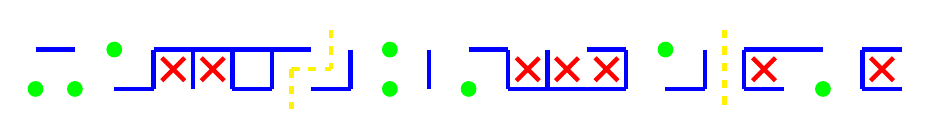
\begin{tikzpicture}[x=0.5cm, y=-0.5cm, ultra thick, blue]
% Walls
    \draw (0,0) -- (1,0);
    \draw (3,0) -- (7,0);
    \draw (11,0) -- (12,0);
    \draw (14,0) -- (15,0);
    \draw (18,0) -- (20,0);
    \draw (21,0) -- (22,0);
    \draw (2,1) -- (3,1);
    \draw (5,1) -- (6,1);
    \draw (7,1) -- (8,1);
    \draw (12,1) -- (15,1);
    \draw (16,1) -- (17,1);
    \draw (18,1) -- (19,1);
    \draw (21,1) -- (22,1);
    \draw (3,0) -- (3,1);
    \draw (4,0) -- (4,1);
    \draw (5,0) -- (5,1);
    \draw (6,0) -- (6,1);
    \draw (8,0) -- (8,1);
    \draw (10,0) -- (10,1);
    \draw (12,0) -- (12,1);
    \draw (13,0) -- (13,1);
    \draw (15,0) -- (15,1);
    \draw (17,0) -- (17,1);
    \draw (18,0) -- (18,1);
    \draw (21,0) -- (21,1);
% Pillars
    \fill[green] (2,0) circle(0.2);
    \fill[green] (9,0) circle(0.2);
    \fill[green] (16,0) circle(0.2);
    \fill[green] (0,1) circle(0.2);
    \fill[green] (1,1) circle(0.2);
    \fill[green] (9,1) circle(0.2);
    \fill[green] (11,1) circle(0.2);
    \fill[green] (20,1) circle(0.2);
% Inner points in accessible cul-de-sacs
    \node at (3.5,0.5) {};
    \node at (4.5,0.5) {};
    \node at (12.5,0.5) {};
    \node at (13.5,0.5) {};
    \node at (14.5,0.5) {};
    \node at (18.5,0.5) {};
    \node at (21.5,0.5) {};
% Entry-exit paths without intersections
    \draw[dashed, yellow] (6.5,0.5) -- (7.5,0.5);
    \draw[dashed, yellow] (6.5,0.5) -- (6.5,1.5);
    \draw[dashed, yellow] (7.5,-0.5) -- (7.5,0.5);
    \draw[dashed, yellow] (17.5,-0.5) -- (17.5,1.5);
\end{tikzpicture}
\end{center}
\vspace*{\fill}

\end{document}
